\documentclass[10pt]{beamer}

\usetheme[progressbar=frametitle,sectionpage=none]{metropolis}
\usepackage{appendixnumberbeamer}

\usepackage{booktabs}
\usepackage[scale=2]{ccicons}

\usepackage{pgfplots}
\usepgfplotslibrary{dateplot}

\usepackage{pgfgantt}
\usepackage{hyperref}

\usepackage[normalem]{ulem}

\usepackage{xspace}
\newcommand{\themename}{\textbf{\textsc{metropolis}}\xspace}

% \definecolor{white}{RGB}{255, 255, 255}
% \definecolor{black}{RGB}{0, 0, 0}
% \definecolor{softgray}{RGB}{240,240,240}
% \definecolor{gray}{RGB}{128,128,128}
\definecolor{oceanblue}{RGB}{0, 119, 190}

% \setbeamercolor{background canvas}{bg=white,fg=black}
% \setbeamercolor{normal text}{fg=black}
% \setbeamercolor{frametitle}{bg=white, fg=black}
\setbeamercolor{progress bar}{fg=oceanblue,bg=oceanblue}

% %For example blocks
% \setbeamercolor{block title example}{fg=red,bg=orange}
% \setbeamercolor{block body example}{fg=cyan,bg=yellow}

% %For alert blocks
\setbeamercolor{block title alerted}{fg=oceanblue}
% \setbeamercolor{block body alerted}{fg=black,bg=softgray}
\setbeamercolor{alerted text}{fg=oceanblue}

% %For blocks
% \setbeamercolor{block title}{fg=white,bg=blue}
% \setbeamercolor{block body}{fg=white,bg=green!40!black}

% Pages
    \setbeamertemplate{footline}{%
       \raisebox{10pt}{\makebox[\paperwidth]{\hfill\makebox[30pt]{\scriptsize\insertframenumber*\ / \inserttotalframenumber*}}}}

\title{GPU Dynamic memory allocation algorithms for Machine Learning: A survey}
\author{Erik H. Wouters, Dragoș Ș. Perju \quad \texttt{ehwo} | \texttt{dsperju}  \texttt{@kth.se}}
\date{November 30, 2018}

\institute{KTH Royal University of Technology \quad Stockholm, Sweden}
% \titlegraphic{\hfill\includegraphics[height=1.5cm]{logo.pdf}}

\begin{document}

\maketitle

% \begin{frame}{Table of contents}
%   \setbeamertemplate{section in toc}[sections numbered]
%   \tableofcontents[hideallsubsections]
% \end{frame}

%\section{Introduction}

\begin{frame}[fragile]{The problem}

\metroset{block=fill}

\begin{exampleblock}{Problem context}
 \begin{itemize}
 \item Dynamic memory allocation;
 \item Different applications use different allocators
     \begin{itemize}
         \item e.g.: \texttt{malloc}, \texttt{jemalloc}, etc.;
     \end{itemize}
 \item Different architectures (CPU vs. GPU) have different issues with allocating dynamically
     \begin{itemize}
         \item e.g.: \texttt{malloc} vs. \texttt{CudaMalloc}.
     \end{itemize}
 \end{itemize}
\end{exampleblock}
\end{frame}

\begin{frame}[fragile]{The problem}

\metroset{block=fill}

\begin{alertblock}{Problem statement}
% We believe that \textbf{machine learning} applications can benefit from using a scientifically chosen dynamic memory allocator, in order to have an improved performance.
 We want to choose the best dynamic memory allocator when used with \textbf{TensorFlow}'s benchmark implementation of \textbf{ResNet-50}, in terms of overall speed, fragmentation and other metrics.
\end{alertblock}
\end{frame}

\begin{frame}[fragile]{The problem}

\metroset{block=fill}

\begin{alertblock}{Problem statement}
% We believe that \textbf{machine learning} applications can benefit from using a scientifically chosen dynamic memory allocator, in order to have an improved performance.
 We want to choose the best dynamic memory allocator when used with \textbf{TensorFlow}'s benchmark implementation of \textbf{ResNet-50}, in terms of overall speed, fragmentation and other metrics.
\end{alertblock}

\begin{exampleblock}{More specifically}
 The memory allocation pattern of \textbf{TensorFlow}'s implementation of \textbf{ResNet-50} is not a great match for the memory allocator TensorFlow uses, we will investigate which previously published dynamic memory allocation algorithms perform better.
\end{exampleblock}

\end{frame}

\begin{frame}[fragile]{The problem}

\metroset{block=fill}

\begin{exampleblock}{More specifically}
We extracted some GPU memory allocators' implementations from the source code of:

\textit{M. Vinkler and V. Havran, “Register efficient dynamic memory allocator for GPUs” , Computer Graphics Forum, vol. 34, no. 8, pp. 143–154, 2015. [Online].} Available: \url{https://onlinelibrary.wiley.com/doi/abs/10.1111/cgf.12666}

TensorFlow uses NVIDIA CUDA as a GPU library, and \texttt{BFCAllocator} or \texttt{CudaMalloc} as the primary dynamic GPU memory allocator.
\end{exampleblock}
\end{frame}

\begin{frame}[fragile]{BFCAllocator}
 \begin{figure}
 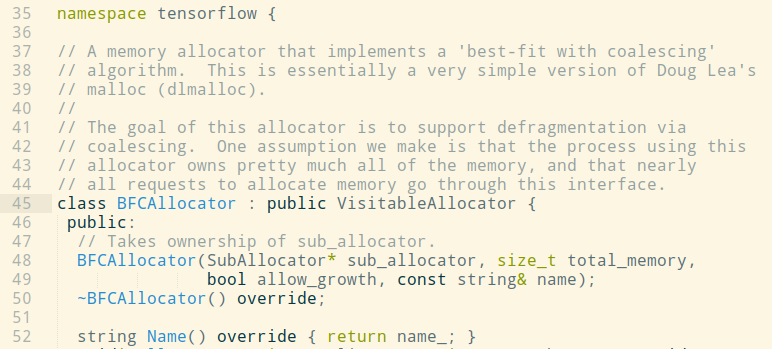
\includegraphics[scale=0.4]{images/BFCAllocator.png}
 \caption{Exerpt from TensorFlow's source code, showing \texttt{BFCAllocator}}
 \end{figure}
\end{frame}

%\begin{frame}[fragile]{The problem}
%
%\metroset{block=fill}
%
%\begin{alertblock}{Problem statement}
% We believe that \texttt{BFCAllocator} is still unsuitable for TensorFlow and Convolutional %Neural Networks. We do not have a \textbf{hypothesis} yet, but we believe another allocation %algorithm can be mainly faster than \texttt{BFCAllocator}.
%\end{alertblock}
%
%\end{frame}

\begin{frame}[fragile]{Goals}

\metroset{block=fill}

\begin{alertblock}{Goals}
%Test different GPU dynamic memory allocation algorithms                           (such as: CudaMalloc and others);
Benchmark such algorithms using a Machine Learning workload (TensorFlow CNN benchmarks).
\begin{enumerate}
    \item Design a repeatable experiment that evaluates the performance of different GPU memory allocation algorithms for the ResNet-50 benchmark. This experiment will be used to validate the hypothesis. 
    \item Understand why these algorithms are faster (or slower).
    \item If we find a faster algorithm, send results and recommendation to the TensorFlow team for study and possible implementation in the release version.
\end{enumerate}

\end{alertblock}
\end{frame}

\begin{frame}[fragile]{Hypothesis}

\metroset{block=fill}

\begin{alertblock}{Hypothesis}
Our hypothesis is that one or more of the algorithms described by Vinkler and Havran perform better as a memory allocator for TensorFlow's implementation of ResNet-50 than the stock \texttt{BFCAllocator} or the standard \texttt{CudaMalloc} does, in terms of overall speed, fragmentation and stability.
\end{alertblock}
\end{frame}

\begin{frame}[fragile]{Problem importance}

\metroset{block=fill}

\begin{exampleblock}{Why is the problem is important to solve}
Improving allocation for \textbf{machine learning} means better performance for the same amount of time and the same amount of energy. 
\end{exampleblock}

\end{frame}

\begin{frame}[fragile]{Methodology}

\metroset{block=fill}

\begin{alertblock}{GPU Dynamic memory allocation algorithms}
 \begin{itemize}
     \item \textbf{CudaMalloc} - proprietary algorithm of NVIDIA;
     \item \textbf{CircularMalloc} - organizes the memory pool as a singly linked list;
     \item \textbf{ScatterAlloc} - can efficiently deal with hundreds of requests in parallel;
     \item \textbf{Halloc} - hashing function to reduce the cost of small memory allocations.
 \end{itemize}
\end{alertblock}

\begin{exampleblock}{TensorFlow CNN benchmark}
 \textbf{ResNet-50} - a deep learning convolutional neural network
\end{exampleblock}

\end{frame}

{
\begin{frame}{Gantt Chart}

\hspace{-1cm}
\begin{ganttchart}[vgrid,today=7,x unit=0.80cm,
            y unit title=0.7cm,
            y unit chart=0.725cm,
            bar label font=\footnotesize,
            milestone label font=\footnotesize,
            group label font=\footnotesize,
            title label font=\footnotesize
]{1}{11}
    \gantttitle{2018}{11} \\
    \gantttitle{Aug}{1}
    \gantttitle{Sep}{4}
    \gantttitle{Oct}{4}
    \gantttitle{Nov}{2} \\
    \gantttitle{W1}{1}
    \gantttitle{W2}{1}
    \gantttitle{W3}{1}
    \gantttitle{W4}{1}
    \gantttitle{W5}{1}
    \gantttitle{W6}{1}
    \gantttitle{W7}{1}
    \gantttitle{W8}{1}
    \gantttitle{W9}{1}
    \gantttitle{W10}{1}
    \gantttitle{W11}{1}
    
    \ganttgroup{Experiment}{2}{9} \ganttnewline
    \ganttgroup{Report}{9}{11} \ganttnewline
    \ganttbar{Tools setup}{3}{9} \ganttnewline
    \ganttbar{Obtain data}{9}{11} \ganttnewline
    \ganttbar{Literature study}{1}{8} \ganttnewline
    \ganttbar{Write report}{9}{11} \ganttnewline
    \ganttmilestone{Project plan 1}{2} \ganttnewline
    \ganttmilestone{Project plan 2}{7} \ganttnewline
    \ganttmilestone{First report}{10}
    \ganttlink{elem5}{elem8} % Write report -> First report
    \ganttlink{elem2}{elem3} % Tools setup -> Obtain data
\end{ganttchart}


\end{frame}
}

{
\begin{frame}{Timeline \& Milestones}

\hspace{-1cm}
\begin{ganttchart}[vgrid,x unit=0.80cm,
            y unit title=0.7cm,
            y unit chart=0.725cm,
            bar label font=\footnotesize,
            milestone label font=\footnotesize,
            group label font=\footnotesize,
            title label font=\footnotesize
]{1}{10}
    \gantttitle{2018}{7}
    \gantttitle{2019}{3} \\
    \gantttitle{Nov}{3}
    \gantttitle{Dec}{4}
    \gantttitle{Jan}{3} \\
    \gantttitle{W12}{1}
    \gantttitle{W13}{1}
    \gantttitle{W14}{1}
    \gantttitle{W15}{1}
    \gantttitle{W16}{1}
    \gantttitle{W17}{1}
     \gantttitle{Christmas}{2}
    \gantttitle{W18}{1}
    \gantttitle{W19}{1}
    
    \ganttgroup{Report}{1}{4} \ganttnewline
    \ganttgroup{Opposition}{2}{6} \ganttnewline
    \ganttbar{Write report}{1}{8} \ganttnewline
    \ganttbar{Write opposition}{2}{4} \ganttnewline
    \ganttmilestone{Opposition}{4} \ganttnewline
    \ganttmilestone{Second report}{4} \ganttnewline
    \ganttmilestone{Third report}{6} \ganttnewline
    \ganttmilestone{Final report \& presentation}{9}
    % Link buldge / Link mid tries not to overlap arrows with each other. It's like spacing for arrows.
    \ganttlink[link bulge=0.7, link mid=0.3]{elem3}{elem4}
    \ganttlink{elem2}{elem5}
    \ganttlink{elem2}{elem6}
    \ganttlink{elem2}{elem7}
    \ganttlink{elem3}{elem7}
\end{ganttchart}

\end{frame}

}

\end{document}
